\section{L05-Macchine termodinamiche}
\subsection{Macchina termodinamica}
Per rappresentare \textbf{macchine termodinamiche} utiliziamo solitamente questa struttura:
\begin{center}
    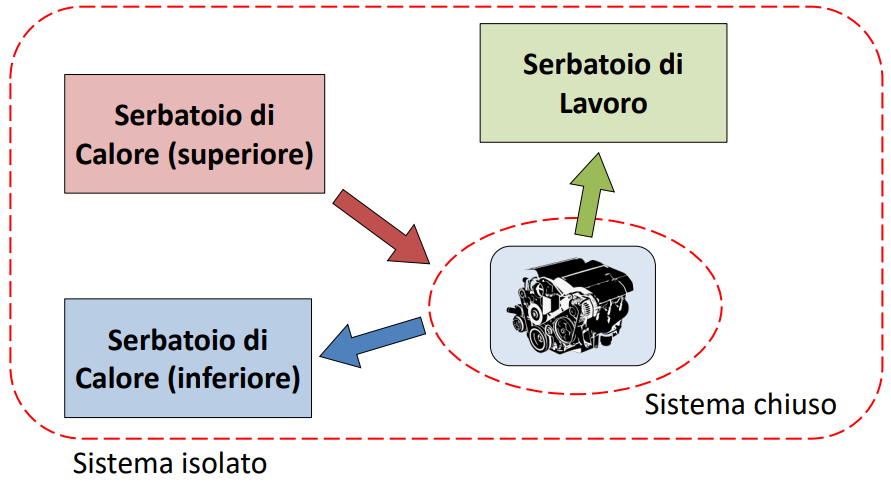
\includegraphics[height=5cm]{../L05/img1.PNG}
\end{center}
La \textbf{macchina termodinamica} è un sistema termodinamico \textbf{composto} e \textbf{isolato}, che, nella sua forma più semplice, è realizzato da:
\begin{itemize}
    \item due serbatoi di calore, uno superiore e uno inferiore;
    \item un serbatoio di lavoro;
    \item una macchina ciclica, che è in grado di produrre od assorbire con continuità lavoro interagendo con il serbatoio di lavoro ed i serbatoi di calore.
\end{itemize}
\subsubsection{Serbatoio di calore}
Il \textbf{serbatoio di calore} è un sistema termodinamico che scambia \textbf{solo calore} con l'esterno senza alterare il suo stato termodinamico (cioè la temperatura e la pressione del serbatoio rimangono costanti, tutto ciò che è al suo interno rimane costante, il suo stato non cambia); gli scambi avvengono con trasformazioni quasi-statiche (\textbf{internamente reversibili}).\newline
\newline
Questa definizione di serbatoio è sinonimo di un sistema \textbf{a massa infinita}: se la massa di un sistema $A$ è enormemente maggiore della massa di un sistema $B$, durante un interazione fra $A$ e $B$, $A$ sembrerà rimanere invariata, poichè tutte le trasformazioni e tutte le grandezze sono legate in proporzione alla massa.\newline
\newline
Un tipico esempio di serbatoio di calore e l'atmosfera terrestre.
\subsubsection{Serbatoio di lavoro}
Il \textbf{serbatoio di lavoro} è un sistema termodinamico che scambia \textbf{solo lavoro} con l'esterno senza alterare il suo stato termodinamico; gli scambi avvengono con trasformazioni quasi-statiche (\textbf{internamente reversibili}).\newline
\newline
Un tipico esempio di serbatoio di lavoro è la rete elettrica.
\subsubsection{Macchina motrice}
Per \textbf{macchina ciclica} si intendono macchine che compiono trasformazioni con stato finale e stato iniziale identici e ripetono $n$ volte tale ciclo.\newline
\newline
Esistono due schemi principali di macchine cicliche: quelle motrici e quelle operatrici. Vediamo la macchina motrice. \newline
\newline
Il \textbf{serbatoio superiore} è a \textbf{temperatura calda} $T_C$ e prende il nome di \textbf{camera di combustione}.\newline
Il serbatoio di calore a $T_C$ e la macchina ciclica, producono un lavoro verso il serbatoio di lavoro e devono rilasciare calore verso un \textbf{serbatoio inferiore} a \textbf{temperatura fredda} $T_F$ che tipicamente è l'\textbf{ambiente}.
\begin{center}
    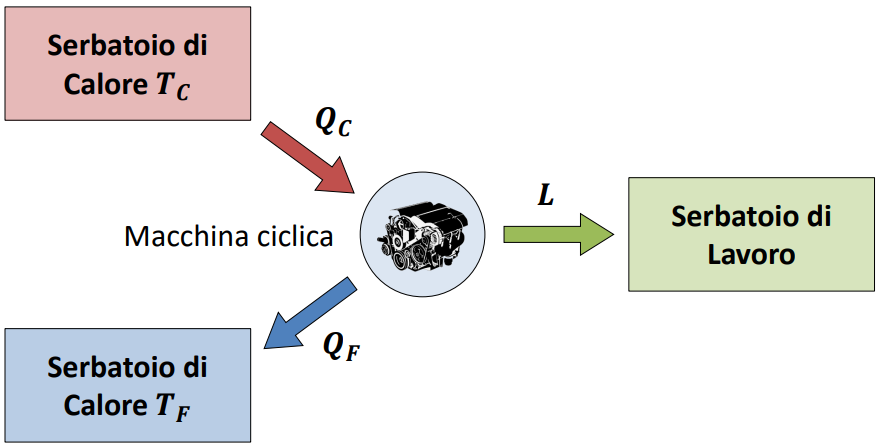
\includegraphics[height=5cm]{../L05/img2.PNG}
\end{center}
Vediamo la macchina motrice da un punto di vista analitico.\newline
Dalle equazioni di bilancio otteniamo:
\[
    \begin{cases}
        \Delta U_Z = 0\\ \Delta S_Z = S_{irr}
    \end{cases} \;\;\;\;\;\;\;\;\;\;\;\;\;\;\; \begin{cases}
        \Delta U_C + \Delta U_F + \Delta U_{SL} + \Delta U_M = 0 \\
        \Delta S_C + \Delta S_F + \Delta S_{SL} + \Delta S_M = S_{irr}
    \end{cases}
\]
Osservando i singoli sottosistemi otteniamo:
\[
    \begin{cases}
        \Delta U_C = Q_C^\leftarrow \\ \Delta S_C = \frac{Q_C^\leftarrow }{T_C}
    \end{cases} \;\;\;\;\; \begin{cases}
        \Delta U_F = Q_F^\leftarrow \\ \Delta S_F = \frac{Q_F^\leftarrow}{T_F}
    \end{cases} \;\;\;\;\; \begin{cases}
        \Delta U_{SL} = - L_{SL}^\rightarrow \\ \Delta S_{SL} = 0
    \end{cases} \;\;\;\;\; \begin{cases}
        \Delta U_M = 0\\ \Delta S_M = 0
    \end{cases}
\]
Per cui deriviamo che
\[
    \begin{cases}
        Q_C^\leftarrow  + Q_F^\leftarrow  - L_{SL}^\rightarrow  = 0\\
        \frac{Q_C^\leftarrow}{T_C} + \frac{Q_F^\leftarrow}{T_F} = S_{irr}
    \end{cases} \;\;\;\;\;\;\;\;\;\; \begin{cases}
        -Q_C + Q_F + L = 0\\
        -\frac{Q_C}{T_C} + \frac{Q_F}{T_F} = S_{irr}
    \end{cases}
\]
\textbf{Rendimento}:\newline
Da queste equazioni ricaviamo che il lavoro è massimo quando il processo è \textbf{reversibile}, per cui il \textbf{rendimento} è
\[
    \eta = \frac{\text{EFFETTO UTILE}}{\text{SPESA}}
\]
La definizione di rendimento si traduce in formule per la macchina motrice così:
\[
    \eta = \frac{L}{Q_C} = 1- \frac{T_F}{T_C} - \frac{T_F}{Q_C} S_{irr} \;\;\;\;\;\;\;\;\;\;\eta_{reversibile} = 1 - \frac{T_F}{T_C}
\]
dove $\eta_{reversibile}$ viene utilizzato per calcolare il rendimento massimo che si può avere.\newline
Queste formule sono valide per serbatoi di calore a temperatura costante, nel momento in cui questa condizione viene meno, non possiamo più usarle, però possiamo sempre usare la definizione di rendimento (effetto utile/ spesa).
\subsubsection{Macchina operatrice}
La \textbf{macchina operatrice} ha un meccanismo opposto alla macchina motrice: usa del lavoro dal \textbf{serbatoio di lavoro} per assorbire calore da un \textbf{serbatoio freddo}, a causa dell'utilizzo di questo lavoro c'è bisogno di rilasciare del calore in un \textbf{serbatoio caldo}.
\begin{center}
    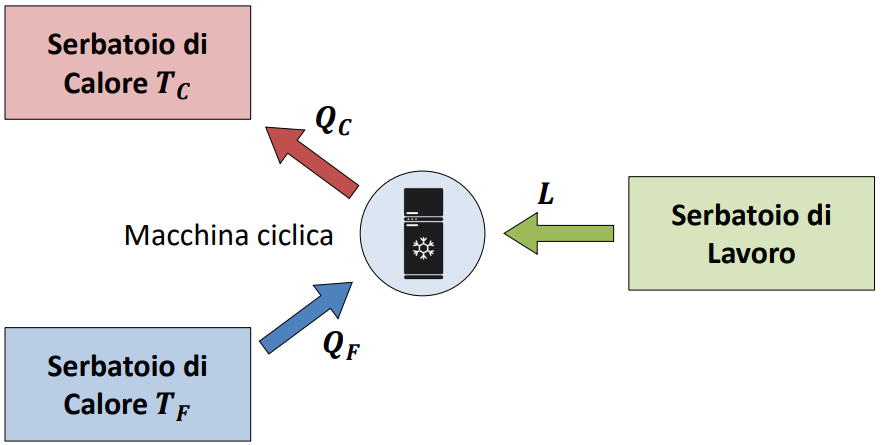
\includegraphics[height=5cm]{../L05/img3.PNG}
\end{center}
Vediamo la macchina operatrice da un punto di vista analitico.\newline
Dalle equazioni di bilancio otteniamo:
\[
    \begin{cases}
        \Delta U_Z = 0\\ \Delta S_Z = S_{irr}
    \end{cases} \;\;\;\;\;\;\;\;\;\;\;\;\;\;\; \begin{cases}
        \Delta U_C + \Delta U_F + \Delta U_{SL} + \Delta U_M = 0 \\
        \Delta S_C + \Delta S_F + \Delta S_{SL} + \Delta S_M = S_{irr}
    \end{cases}
\]
Osservando i singoli sottosistemi otteniamo:
\[
    \begin{cases}
        \Delta U_C = Q_C^\leftarrow \\ \Delta S_C = \frac{Q_C^\leftarrow }{T_C}
    \end{cases} \;\;\;\;\; \begin{cases}
        \Delta U_F = Q_F^\leftarrow \\ \Delta S_F = \frac{Q_F^\leftarrow}{T_F}
    \end{cases} \;\;\;\;\; \begin{cases}
        \Delta U_{SL} = - L_{SL}^\rightarrow \\ \Delta S_{SL} = 0
    \end{cases} \;\;\;\;\; \begin{cases}
        \Delta U_M = 0\\ \Delta S_M = 0
    \end{cases}
\]
Per cui deriviamo che
\[
    \begin{cases}
        Q_C^\leftarrow  + Q_F^\leftarrow  - L_{SL}^\rightarrow  = 0\\
        \frac{Q_C^\leftarrow}{T_C} + \frac{Q_F^\leftarrow}{T_F} = S_{irr}
    \end{cases} \;\;\;\;\;\;\;\;\;\; \begin{cases}
        Q_C - Q_F - L = 0\\
        \frac{Q_C}{T_C} - \frac{Q_F}{T_F} = S_{irr}
    \end{cases}
\]
\textbf{L'unica cosa che cambia rispetto alla macchina motrice sono i segni}.\newline
\newline
\textbf{Efficienza o COP (coefficient of performance)}:\newline
Il lavoro è minimo quando il processo è \textbf{reversibile}, per cui l'\textbf{efficienza} è
\[
    \epsilon = \frac{\text{EFFETTO UTILE}}{\text{SPESA}}
\]
Vediamo ora la formula dell'efficienza nei casi particolari di macchina operatrice \textbf{frigorifera} e \textbf{pompa di calore}:\newline
\textbf{Macchina frigorifera}:
\[
    \epsilon_F = \frac{Q_F}{L} = \frac{T_F}{T_C - T_F + \frac{T_CT_FS_{irr}}{Q_F}} \;\;\;\;\;\;\;\;\;\; \epsilon_{F,reversibile} = \frac{T_F}{T_C-T_F}
\]
dove $\epsilon_{reversibile}$ viene utilizzato per calcolare l'efficienza massima che si può avere.\newline
\textbf{Pompa di calore}:
\[
    \epsilon_P = \frac{Q_C}{L} = \frac{T_C}{T_C - T_F + \frac{T_CT_FS_{irr}}{Q_C}} \;\;\;\;\;\;\;\;\;\; \epsilon_{P,reversibile} = \frac{T_C}{T_C-T_F}
\]
dove $\epsilon_{reversibile}$ viene utilizzato per calcolare l'efficienza massima che si può avere.\newline
\newline
Queste formule sono valide per serbatoi di calore a temperatura costante, nel momento in cui questa condizione viene meno, non possiamo più usarle, però possiamo sempre usare la definizione di efficienza (effetto utile/ spesa).
\newline
\newline
C'è un legame fra l'efficienza della macchina frigorifera e l'efficienza della pompa di calore:
\[
    \epsilon_P = \frac{Q_C}{L} = \frac{Q_F+L}{L} = \epsilon_F + 1
\]
\subsubsection{Macchina motrice con serbatoio caldo a massa finita}
Fino ad ora abbiamo analizzato il comportamento di macchine termodinamiche con serbatoi a massa infinita e quindi temperatura costatne. Vediamo ora il ragionamento che sta sotto l'analisi di macchine motrici con serbatoio caldp a \textbf{massa finita}.\newline
\newline
Per semplificare la trattazione analiziamo \textbf{Macchina motrice con serbatoio caldo a massa finita contenente liquido incomprimibile perfetto} (vediamo il caso con liquido incomprimibile perfetto, ma questo dettaglio ha un impatto irrilevante sulla trattazione, lo usiamo sol oper semplicità di esposizione, si può rieseguire il ragionamento anche con gas perfetti e altro ancora\dots).\newline
\newline
Dalle equazioni di bilancio otteniamo:
\[
    \begin{cases}
        \Delta U_Z = 0\\ \Delta S_Z = S_{irr}
    \end{cases} \;\;\;\;\;\;\;\;\;\;\;\;\;\;\; \begin{cases}
        \Delta U_C + \Delta U_F + \Delta U_{SL} + \Delta U_M = 0 \\
        \Delta S_C + \Delta S_F + \Delta S_{SL} + \Delta S_M = S_{irr}
    \end{cases}
\]
Nel serbatoio a caldo la temperatura iniziale è maggiore di quella finale ($T_1 > T_2$), l'altro serbatoio rimane invece a temperatura costante, per cui:
\[ 
    \begin{cases}
        \Delta U_{C,12} = Mc(T_2 -T_1)\\ \Delta S_{C,12} = Mcln \frac{T_2}{T_1}
    \end{cases}\;\;\;\;\; \begin{cases}
        \Delta U_F = Q_F^\leftarrow \\ \Delta S_F = \frac{Q_F^\leftarrow}{T_F}
    \end{cases} \;\;\;\;\; \begin{cases}
        \Delta U_{SL} = - L_{SL}^\rightarrow \\ \Delta S_{SL} = 0
    \end{cases} \;\;\;\;\; \begin{cases}
        \Delta U_M = 0\\ \Delta S_M = 0
    \end{cases}
\]
Per cui deriviamo che
\[
    \begin{cases}
        Mc(T_2-T_1) + Q_f^\leftarrow - L_{SL}^\rightarrow  = 0\\
        Mc ln \frac{T_2}{T_1} + \frac{Q_F^\leftarrow}{T_F} = S_{irr}
    \end{cases} \;\;\;\;\;\;\;\;\;\; \begin{cases}
        Mc(T_2-T_1) + Q_F + L = 0\\ Mc ln \frac{T_2}{T_1} + \frac{Q_F}{T_F} = S_{irr}
    \end{cases}
\]
\textbf{Caso reversibile} $S_{irr} = 0$:
$Q_C^\leftarrow =  Mc(T_2-T_1)$ negativo uscente; \newline
$Q_C =  Mc(T_2-T_1)$ valore assoluto; \newline
\newline
$Q_F^\leftarrow  = - Mc T_F ln \frac{T_2}{T_1} = Mc T_F ln \frac{T_1}{T_2}$ positivo entrante;\newline
$Q_F = Mc T_F ln \frac{T_1}{T_2}$ valore assoluto.\newline
\newline
$L^\rightarrow  = Q_C^\leftarrow  + Q_F^\leftarrow  = Mc(T_2 -T_1) + Mc T_F ln \frac{T_1}{T_2}$ negativo entrante;\newline
$L = Q_C- Q_F = Mc (T_1-T_2) - McT_F ln \frac{T_1}{T_2}$ valore assoluto.\newline
\newline
Rendimento $\eta = \frac{L}{Q_C}$ e $\eta_{rev} = \frac{L_{rev}}{Q_C}$.\newline
\newline
\textbf{Rendimento di secondo principio per la macchina motrice}:
\[
    \eta_{II} = \frac{\eta}{\eta_{rev}} = \frac{L}{L_{rev}}
\]
\textbf{Rendimento di secondo principio per la macchina operatrice}:
\[
    \eta_{II} = \frac{\epsilon}{\epsilon_{rev}} = \frac{L_{rev}}{L}
\]